\documentclass{standalone}
\usepackage{tikz}
\usepackage{pgfplots}
\usetikzlibrary{decorations.pathreplacing}
%\usepgfplotslibrary{external}
%\tikzexternalize

% http://tex.stackexchange.com/questions/205549/getting-pictures-from-tikzit-to-latex-and-seeing-them-in-pdf-format
%% -------------------------------------- Declare the layers
\pgfdeclarelayer{nodelayer}
\pgfdeclarelayer{edgelayer}
\pgfdeclarelayer{gridlayer}
\pgfsetlayers{gridlayer,edgelayer,nodelayer,main}

%% -------------------------------------- Declare the styles
\tikzstyle{node}=[circle,draw=black,line width=0.8 pt]
\tikzstyle{smallnode}=[circle,fill=white,draw=black,scale=.75,inner sep=1pt]
\tikzstyle{uvnode}=[circle,draw=none,inner sep=0pt,minimum size=0pt]
\tikzstyle{smalllabel}=[draw=none,scale=.75,inner sep=1pt]

\tikzstyle{towernode}=[circle,draw=black,scale=.75,inner sep=2pt]
\tikzstyle{virtualnode}=[circle,draw=black,dashed,scale=.75,inner sep=2pt]
\tikzstyle{pillarnode}=[circle,fill=black,draw=black,scale=.75,inner sep=2pt]

\tikzstyle{directededge}=[->, thick]
\tikzstyle{undirectededge}=[]
\tikzstyle{undirectededgethick}=[thick]
 \tikzstyle{virtualedge}=[thick,dashed]


%\tikzset{node/.style={thick,shape=circle}}
%\tikzset{label/.style={}}
%\tikzset{edge/.style={->,thick}}
%% --------------------------------------------------------


\begin{document}
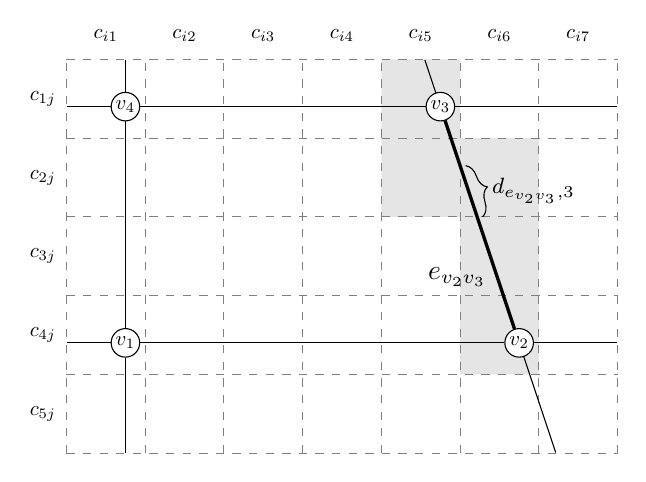
\begin{tikzpicture}

	\begin{pgfonlayer}{gridlayer}
	
		\foreach \xa/\ya/\xb/\yb in {1/3/2/4,1/2/2/3,2/2/3/3,2/1/3/2, 2/1/3/2, 2/0/3/1} {
				\draw[step=1.0,thin,draw=none,fill=black!10!white,dashed] (\xa,\ya) grid (\xb,\yb) rectangle (\xa,\ya);
		}
		
		\foreach \y [count=\i] in {3.5,2.5,...,-0.5} {
			\node[style=smalllabel] (aly\i) at (-3.3,\y) {$c_{\i j}$};
		}
		
		\foreach \x [count=\j] in {-2.5,-1.5,...,3.5} {
			\node[style=smalllabel] (alx\j) at (\x,4.3) {$c_{i\j}$};
		}
		
		\draw[step=1.0,thin,gray,dashed] (-3,-1) grid (4,4);
	\end{pgfonlayer}
	
	\begin{pgfonlayer}{nodelayer}
		\node [style=smallnode] (0) at (-2.25, 0.4) {$v_1$};
		\node [style=smallnode] (1) at (2.75, 0.4) {$v_2$};
		\node [style=smallnode] (2) at (-2.25, 3.4) {$v_4$};
		\node [style=smallnode] (3) at (1.75, 3.4) {$v_3$};
		\node [style=uvnode] (4) at (3.21667, -1) {};
		\node [style=uvnode] (5) at (-2.25, -1) {};
		\node [style=uvnode] (7) at (4, 3.4) {};
		\node [style=uvnode] (8) at (4, 0.4) {};
		\node [style=uvnode] (9) at (-2.25, 4) {};
		\node [style=uvnode] (10) at (1.55, 4) {};
		\node [style=uvnode] (11) at (-3, 0.4) {};
		\node [style=uvnode] (12) at (-3, 3.4) {};
		
		%\draw [decorate,decoration={brace,amplitude=5pt},xshift=2pt,yshift=0pt]  (2.21667,2) -- (2.55,1) node [black,midway,right, xshift=2] {\footnotesize$d_{e,2}$};
		
		\draw [decorate,decoration={brace,amplitude=5pt},xshift=2pt,yshift=0pt]  (2,2.65) -- (2.21667,2) node [black,midway,right, xshift=3] {\footnotesize$d_{e_{v_2v_3},3}$};
		
	\end{pgfonlayer}
	\begin{pgfonlayer}{edgelayer}
		\draw [style=undirectededge] (2) edge (0);
		\draw [style=undirectededge] (0) edge (1);
		\draw [style=undirectededge,very thick] (1) edge node[near start,left]{$e_{v_2v_3}$} (3);
		\draw [style=undirectededge] (3) edge (2);
		\draw [style=undirectededge] (1) edge (4);
		\draw [style=undirectededge] (5) edge (0);
		\draw [style=undirectededge] (1) edge (8);
		\draw [style=undirectededge] (7) edge (3);
		\draw [style=undirectededge] (9) edge (2);
		\draw [style=undirectededge] (10) edge (3);
		\draw [style=undirectededge] (11) edge (0);
		\draw [style=undirectededge] (12) edge (2);
	\end{pgfonlayer}
\end{tikzpicture}
\end{document}
